\section{How could one attack a HSM?}
\begin{frame}{How could one attack a HSM?}
    \begin{wide}
        Through the communication channel and audited software, there should be no logical way to attack a HSM. However, there are some physical attacks that could be attempted:
            \begin{itemize}
                \item Power monitoring
                \item Cold boot
                \item Probing
                \item RNG seeding
            \end{itemize}
    \end{wide}
\end{frame}
\begin{frame}{Power monitoring}
    \begin{wide}
        \begin{block}[Attack]
            When a key is used in binary form, the encryption boils down to "if bit is 1, do this, if bit is 0, do that". When "this" and "that" have different power consumption, an attacker could monitor the power consumption of the HSM and deduce the key.
        \end{block}
        \begin{block}[Defense]
            The power consumption must be decoupled from the operations performed. Possible solutions are:
            \begin{itemize}
                \item Insert random delays
                \item Add dummy operations
                \item Add noise or smooth the power consumption
            \end{itemize}
        \end{block}
    \end{wide}
\end{frame}
\begin{frame}{Cold boot}
    \begin{wide}
        \begin{block}[Attack]
            After powering off the HSM, the RAM is still readable for a short period of time. This time can be extended by cooling the RAM.
        \end{block}
        \begin{block}[Defense]
            The RAM must be cleared when the HSM is powered off. Possible solutions are:
            \begin{itemize}
                \item Use of a battery to ensure a proper shutdown
                \item The RAM must be securely overwritten
                \item Ensure self destruction at extreme low temperatures
            \end{itemize}
        \end{block}
    \end{wide}
\end{frame}
\begin{frame}{Probing}
    \begin{wide}
        \begin{block}[Attack]
            An attacker could probe the HSM with a needle and measure the voltage on the needle. This could give the attacker information about the internal workings of the HSM.
        \end{block}
        \begin{block}[Defense]
            The HSM must detect physical intrusion. Possible solutions are:
            \begin{itemize}
                \item Encase the HSM in a harden shell
                \item Use a vibration sensor to detect probing
                \item Surround the HSM with a mesh that will short-circuit the HSM when probed
            \end{itemize}
        \end{block}
    \end{wide}
\end{frame}
\begin{frame}{RNG seeding}
    \begin{wide}
        \begin{block}[Attack]
            If the RNG of the HSM is depending on some outside influence, an attacker could manipulate the RNG and predict the keys generated by the HSM.
        \end{block}
        \begin{block}[Defense]
            The RNG must be truly random. Possible sources are:
            \begin{columns}[c]
                \column{0.45\textwidth}
                \begin{itemize}
                    \item Decay of a radioactive isotope
                    \item brownian motion
                    \item Use of a quantum RNG
                \end{itemize}
                \column{0.45\textwidth}
                        \begin{figure}
                            \centering
                            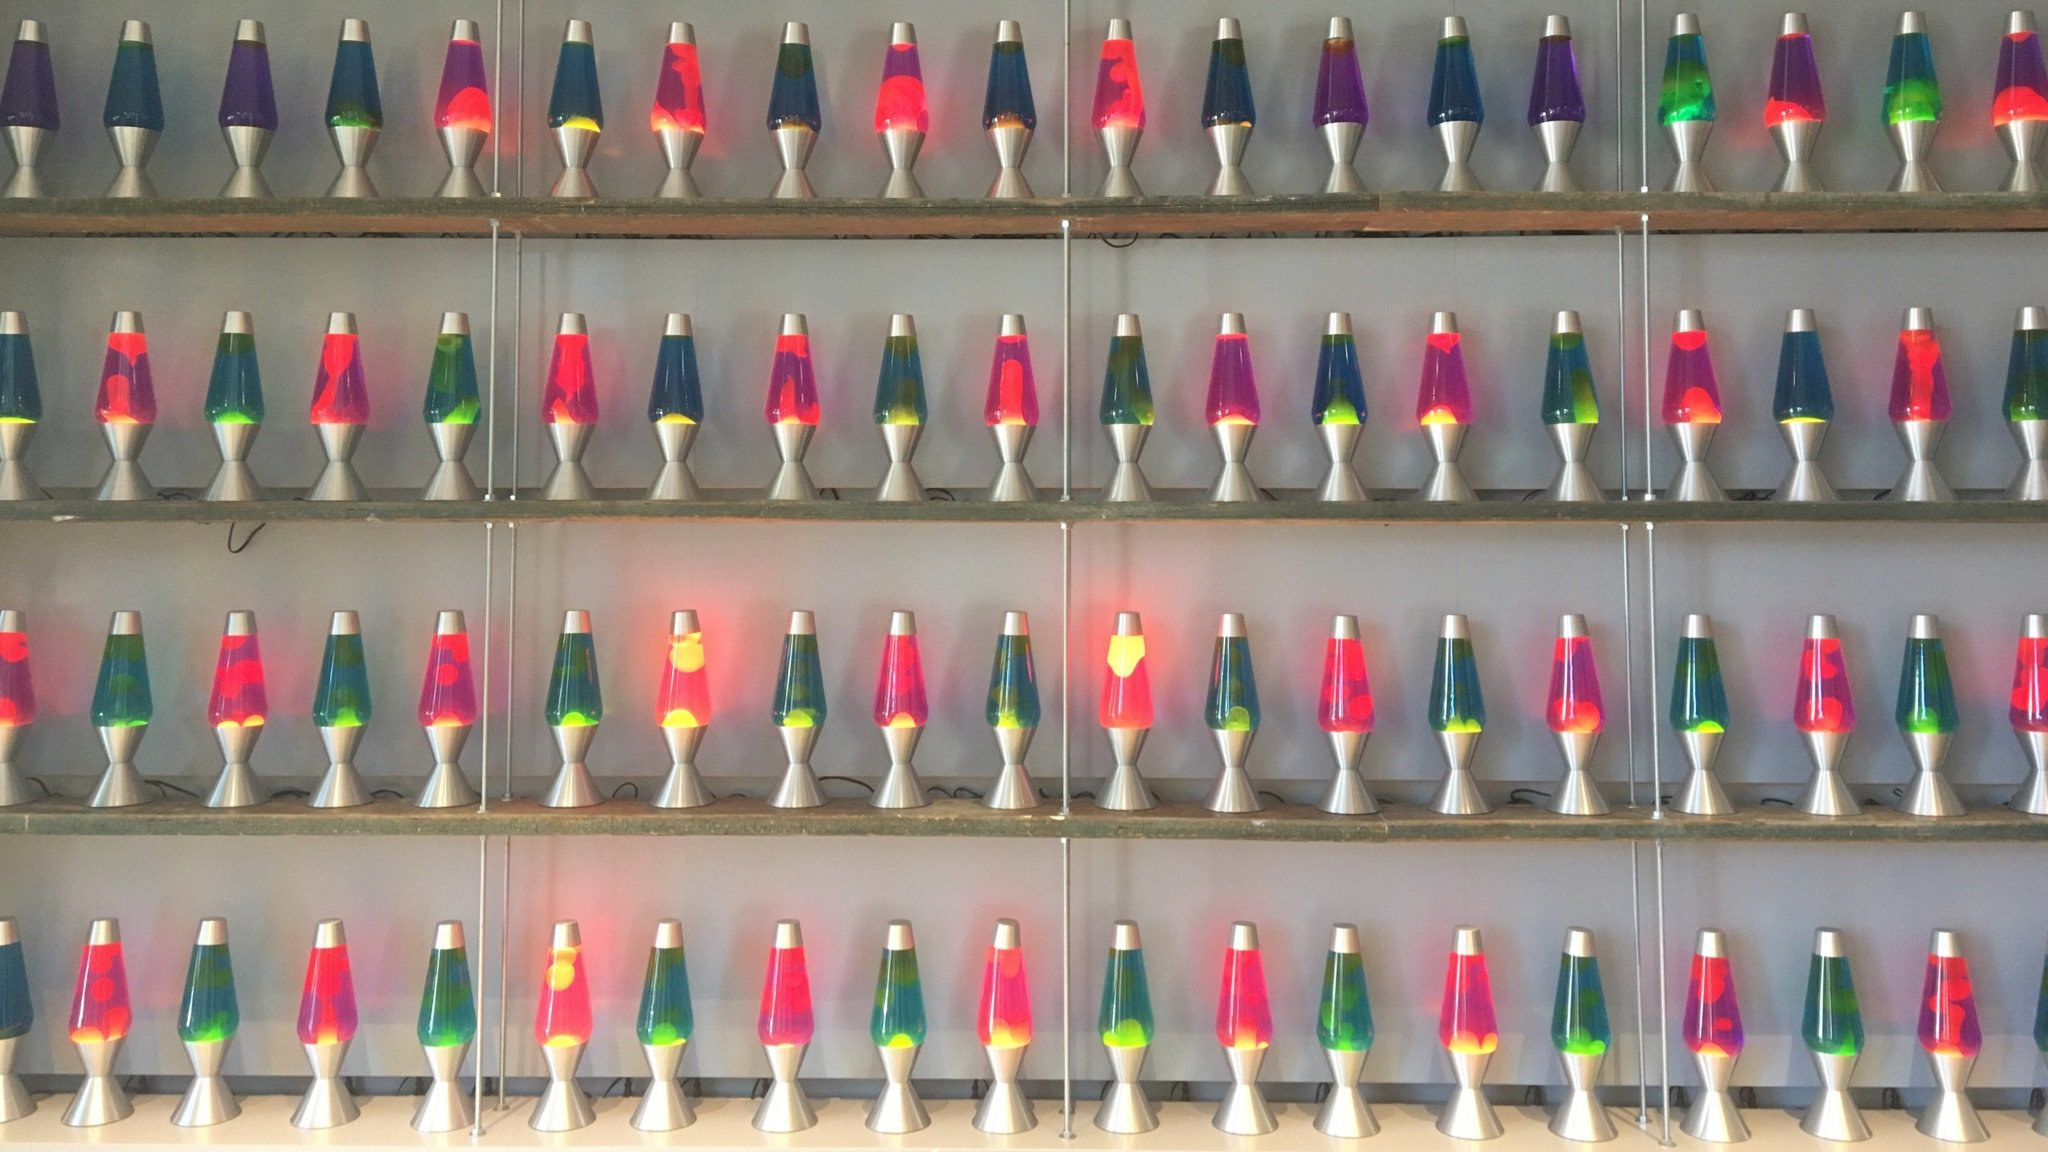
\includegraphics[width=0.4\textwidth]{figures/lava-lamps.jpg}
                            \caption{"The Wall of Entropy" by CloudFlare\footnotemark[3].}
                        \end{figure}

                \end{columns}
        \end{block}
        \footnotetext{3: \fullcite{cloudflare}}
    \end{wide}
\end{frame}